\documentclass[l4proj.tex]{subfiles}
\begin{document}

This chapter discusses the different means of evaluation that were conducted on the RViT project and discusses the results obtained from these.

\section{Testing}
Two sets of unit test suites were created to ensure the code worked as expected. These tests were incorporated into the continuous integration pipelines found on RViT's GitHub repository.

To test the Django REST API, a number of unit test suites were created using Python's unittest library. These tests were created as the code base was developed and were particularly helpful when diagnosing issues regarding the expected behaviour of the API. As seen in \textbf{Fig. \ref{fig:django unit tests}}, these tests cover $96\%$ of statements found in the Django code base. For conciseness the statement coverage of the migrations were edited out, however these were all $100\%$. The one downside to the high code coverage of these tests was their brittleness. This was noted particularly in the latter stages of development when the administration side of the application was created, as multiple models were refactored. This led to tests breaking for the majority of the edited models, and slowed down development while the tests were repaired.
 

\begin{figure}[h!]
\begin{center}
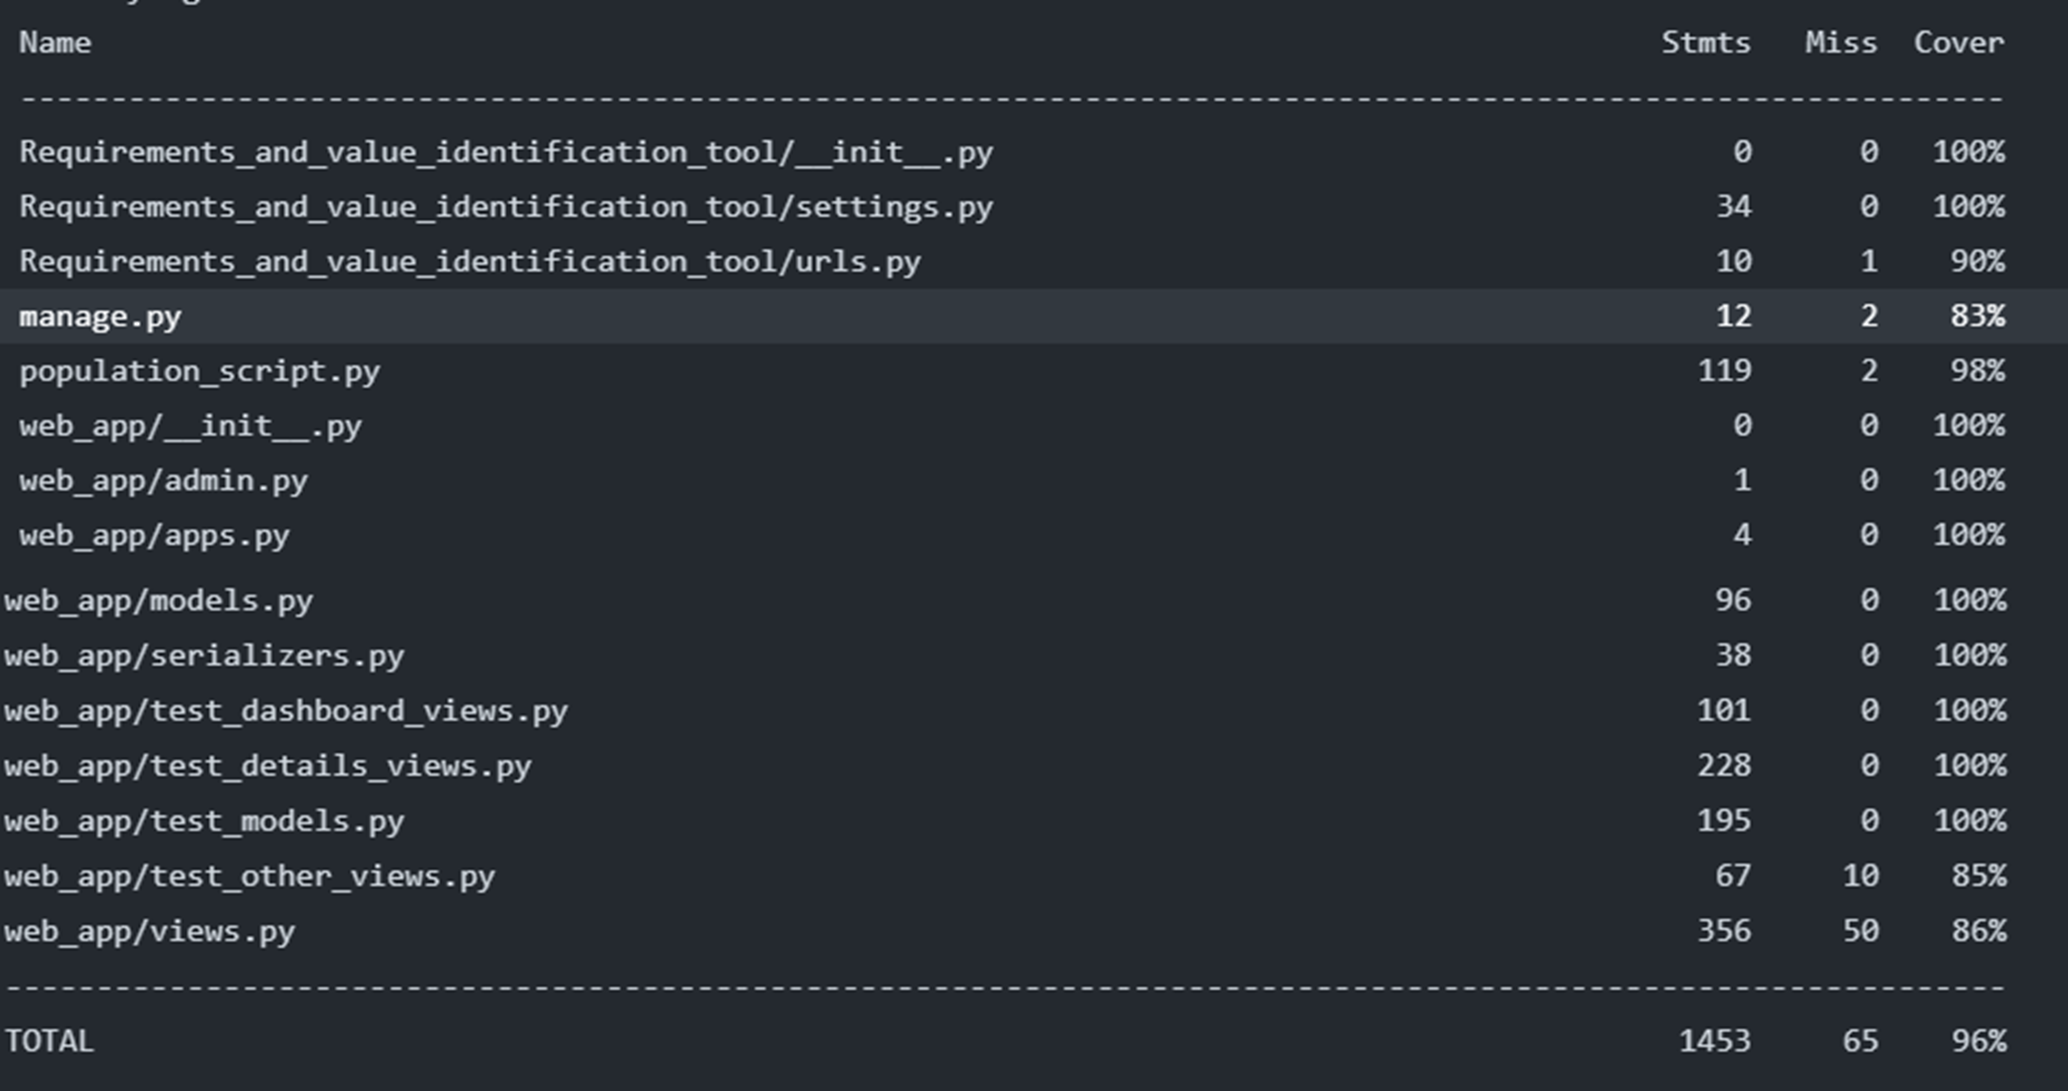
\includegraphics[scale=0.5]{dissertation/images/DjangoUnitTests.png}
\caption{Django unit tests code coverage not including migrations for brevity.}
\label{fig:django unit tests} 
\end{center}
\end{figure}

Unlike the API, the front-end was tested manually for the majority of its development. This was due to frequent changes to design and the repeated refactoring of the React code base. Towards the end of the project however, it was decided that some unit tests should be written to aid in future development. Due to the scope of the React code base, there was not enough time to fully test all components and helper functions. It was decided to prioritise the form-based components, as accidental changes to these files could introduce further problems throughout the code base.

The React Testing Library was chosen to test the React code base. This is a react-specific testing library built on top of the DOM Testing Library (\cite{ReactTestingLibrary})). This testing approach focuses on testing the user interface through interactions with the components rather than testing the underlying implementation, leading to more maintainable tests. As the React Testing Library is framework agnostic (\cite{ReactTestingLibrary}) Jest was used. Jest was chosen for a number of reasons, not only is it capable of generating code coverage reports and provides easy to use mocking functionality, but the author was also familiar with the framework, meaning tests could be developed quickly. As seen in  \textbf{Fig. \ref{fig:react unit tests}}, in total 23 test suites were created, one for each component tested, covering $30\%$ of the lines found in the React code base.

\begin{figure}[h!]
\begin{center}
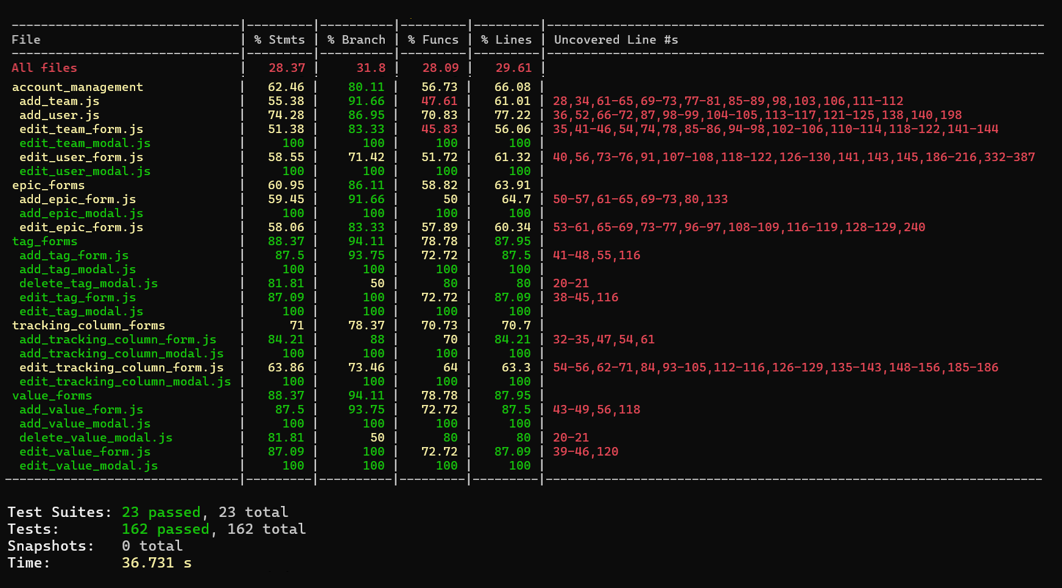
\includegraphics[scale=0.4]{dissertation/images/ReactUnitTests.png}
\caption{React unit tests code coverage not including untested files for brevity.}
\label{fig:react unit tests} 
\end{center}
\end{figure}


\section{Performance and accessibility evaluation}
Requirement \textbf{MH.20} states that the produced application must have quick load times and perform well in order to ensure ease of use. To evaluate this Lighthouse was used. This is an automated tool that can be used to evaluate the performance and accessibility of a web page, as well as how closely the page follows best development practices \cite{LighthouseOverview}. To investigate if there were any changes in these measures based on the browsers used, two different browsers were used in testing: Google Chrome and Microsoft Edge. It was noticed that the performance metric varied between runs, so each page was tested three times per browser and results were averaged with the metric measurements rounded to the nearest whole number. 


As can be seen in \textbf{Table \ref{perfomance-metrics-table}}, only a small subset of the created web pages were chosen to be tested. The pages chosen were the ones that contained high numbers of API calls, or had a significant quantity of components to be displayed, as these were likely to have the slowest performance. 

\begin{center}
\begin{table}[h!]
\begin{tabular}{| c | c | c | c | c |}
\hline
 Web Page & Performance & Accessibility & Best Practices & Speed Index (seconds) \\ 
 \hline
 Epics Dashboard & 94 & 91 & 96 & 0.95 \\  
 Tag Dashboard & 100 & 86 & 96 & 0.48    \\
 Tracking Dashboard  & 99 & 91 & 96 & 0.77  \\
 View Teams & 99 & 93 & 96 & 0.42 \\
 View Users & 98 & 88 & 96 & 0.53\\
 \hline
\end{tabular}
\caption{Evaluation results averaged over the two web browsers used. Metrics are scored out of 100.}
\label{perfomance-metrics-table}
\end{table}
\end{center}

According to the Lighthouse documentation, scores between 90 to 100 are deemed as good, while between 50 to 89 means improvement is needed, and scores of 49 and below are deemed poor (\cite{LighthouseColourCoding}). As all performance metrics are above 94, requirement \textbf{MH.20} has been met. However, future improvements can still be made. Using a hosting platform with dedicated servers or better performance could greatly lower the speed index of the application, providing users with a smoother experience. 

Through the accessibility metric, it was also noticed that some colour contrasts used in the application did not meet the WCAG text contrast guidelines (\cite{WCAGContrastGuidelines}). This can be fixed by re-theming the application with colours that ensure these guidelines are met. It was noticed that the custom colour of components such as epics also directly impact the accessibility of the page. The idea behind the custom colour choice was that this would allow for team members with visual impairments to be accounted for while creating these components. However, to ensure accessibility standards are met, future work could include creating an accessibility meter of sorts so teams could be made aware of how possible colour choices may affect the readability of components.


\section{Security Evaluation}
The requirement \textbf{MH.21} states that the application created must be secure to ensure users are protected while using the application. Although Google Lighthouse includes some basic security checks to evaluate if best practice has been followed (\cite{LighthouseOverview}), it was felt that these checks did not fully test the security of the application, so further evaluations were carried out. 

The JFrog Visual Studio extension was used to scan the RViT's dependencies to identify any vulnerable components. In total, nine vulnerable dependencies in the package.json were found, with the securities ranging from medium to critical. These vulnerabilities were examined, and it was found that most of these were indirect vulnerabilities with the only critical vulnerability being EJS, a popular Node.js templating library used in the project. No changes to the code base were made as a result of this security check, as all vulnerable dependencies found were used significantly in the project. In the future, dependencies should be checked with JFrog and any vulnerabilities evaluated before they are on-boarded to the project. 

Snyk, a code vulnerability scanner, was then used to analyse RViT's code base and identify any security flaws. This tool was chosen as it provided a good range of tests at the free tier for individual developers and small teams, unlike other tooling which had either no free tier or extremely limited free tests. In total 147 issues were found in the code, however 109 of these issues were found in the virtual environment that had been created to run the Django project locally. A total of 35 issues were found in the core RViT project code base, of which, 7 were of medium severity, and the remaining 28 low severity. Four of the medium severity issues identified were 'Cross-site scripting' vulnerabilities, where data from the database flowed into an attribute which is dynamically constructed on the client side, which could result in a DOM based cross-site scripting attack. The other three medium security errors were flagged as 'use of hardcoded credentials', where the password state variable used for form validation checking was set to 'valid' or 'invalid'. These vulnerabilities should be ignored as they were incorrectly flagged by the application. The remaining 28 low vulnerability issues found were also flagged as 'use of hardcoded credentials', where mock users were set up to carry out front and back end testing. As these were required for testing, they can also be ignored. Future development should consider a solution for the cross-site Scripting vulnerabilities and use tooling like Snyk throughout development to ensure code is kept as secure as possible.


\section{User Evaluation}
A user evaluation was carried out in order to understand how well RViT had fulfilled the requirements specified at the beginning of the project. The evaluation aligned with the University of Glasgow's School of Computing Science ethics checklist and a signed copy of this can be found in \textbf{Appendix \ref{app: ethics checklist}}


\subsection{Evaluation methodology}
As the majority of the participants would be completing the evaluation remotely, an online survey was deemed to be the best choice, as the participants would be able to complete it in their own time.

To limit the question fatigue participants experienced, the survey was designed to take roughly 30 minutes to complete. Due to this time constraint, it would be impossible to ask the participants to explore and evaluate the full functionality of RViT. Therefore, they were asked to complete three sections of tasks designed to cover the core website functionality, especially the Epics, Tag, and Tracking Dashboards. The aim was to mimic the workflow of a typical user, so multiple small tasks were designed for each section.

Firstly, the participants were given an information sheet to read before they consented to participate in the study. This information sheet asked them to familiarise themselves with the help documentation and asked them to use dummy data while completing the survey.

For each section of tasks, participants were asked to complete the specified set of tasks before filling out a series of Likert scale questions, followed by an open-ended text question on additional feedback.

The first section of tasks were designed to evaluate the admin user workflow. The participants were asked to sign up with an organisation and admin account then add a team member user to two newly-created teams. They were then asked a series of Likert scale questions on how challenging they found each task, before being asked an open-ended question on additional feedback. In the next section, the participants were asked to log in with the newly created user to complete a set of tasks using the Epics and Tag Dashboard. The participants were then asked a series of Likert scale questions on how challenging they found the tasks and how much they agreed or disagreed with a number of statements surrounding the functionality they had used. As before, they were then also asked if they had any additional comments on the pages used. In the final task section, participants were asked to use their newly created stories in the Tracking Dashboard. Like the previous section, they were asked to rate how challenging they found the tasks as well as their opinion on the pages used in this section. As with the other sections they were then asked for any additional feedback.

Finally, to obtain the most amount of feedback possible, the participants were asked to complete four open-ended optional text responses. The first of these responses asked participants to compare RViT to any similar tooling they had used, while the second question asked the participants if they had any suggestions for future work or improvements. The third question asked if the participants had any further feedback they wanted to specify, and the final question asked if the participants had experienced any errors or bugs in their time using RViT. The full set of survey questions can be found in \textbf{Appendix \ref{app: user eval survey}}.


\subsection{Participant recruitment}
As RViT was designed to be an application primarily used by agile teams and software developers, it was deemed necessary that only software developers were recruited to carry out the user evaluation. The participants were recruited through convenience sampling with developers who the author knew asked to take part. In total 20 participants from four different companies were recruited for the study, all of whom were software developers with at least a year of industry experience. Four of these developers who were willing to give up more of their time were asked to participate in a pilot study while the other sixteen participated in the finalised study.

It was noted that all participants knew the author, so courtesy bias could occur. To attempt to mitigate this, all participants were assured that all feedback they could provide was helpful, even if it was negative.


\subsection{Pilot Study}
Prior to the full-scale user evaluation being conducted, a pilot study took place. Four developers were recruited to run through the original user evaluation survey to determine if the survey was understandable and completable within the half an hour time constraint. In order to understand the participant's thought processes, the participants were observed during the pilot study and asked to narrate their thoughts. Once a participant had completed the survey, they were asked in more detail about certain challenges they faced, in order to pinpoint the underlying issues. 

As a result of this pilot study, some of the tasks were re-worded based on participant feedback. The order of some tasks were also changed to flow more aligned to the typical developer experience. It was also decided to make all the open-ended text responses optional based on the feedback received. A small username bug was also noticed here and was resolved before the full-scale evaluation was held.

There were also some design changes made after the pilot study. All four participants required prompting to understand how they could change teams, so this section was made larger and mouse-hover feedback was added. Once this design change was implemented the participants were then asked to provide feedback on the new design and some more tweaks were made. Three of the four participants also struggled to find out how to edit a tracking column, so they were asked for suggested improvements and mouse-hover feedback was added. Some other minor changes were made based on the participants' feedback, such as changing the priority labels to be displayed in upper case and changing the order of the add user form fields.

It was noted during observation that the majority of developers failed to thoroughly read the help documentation or evaluation tasks before interacting with the website and on occasion had to be prompted to re-read a task. All the participants of the pilot study completed the survey in 25 to 35 minutes, so the suggested time frame of 30 minutes was deemed appropriate.


\subsection{Results}
In the full-scale user evaluation, it was noticed that many of the participants took longer than the suggested 30 minutes when completing the survey. When looking into the activity logs to determine the cause of this, it was noticed that these participants conducted extra tests on their own. For instance, one participant attempted to use SQL injections in various areas of the code while another set up many more epics and stories than were required for the evaluation. 

To identify trends and themes in the open-ended text-based questions, qualitative coding was used. As it was not clear what responses the participants would give, an inductive approach to coding responses was used where codes were created based on the data gathered. Coding was conducted manually as 16 surveys had to be analysed. The full list of qualitatively coded text responses can be found in \textbf{Appendix \ref{app: qualitative coding}}

\textbf{Admin Workflow Section}\\
As seen in \textbf{Fig. \ref{fig:admin task graph}}, the majority of users found the admin section tasks to be not at all challenging. However, two participants found the organisation sign up and creating a user tasks moderately challenging. When analysing the text responses provided in this section, this seemed to be due to the users remaining on the form page after its submission rather than being redirected to different pages, with five of the 16 participants highlighting this as an issue.

\begin{figure}[h!]
\begin{center}
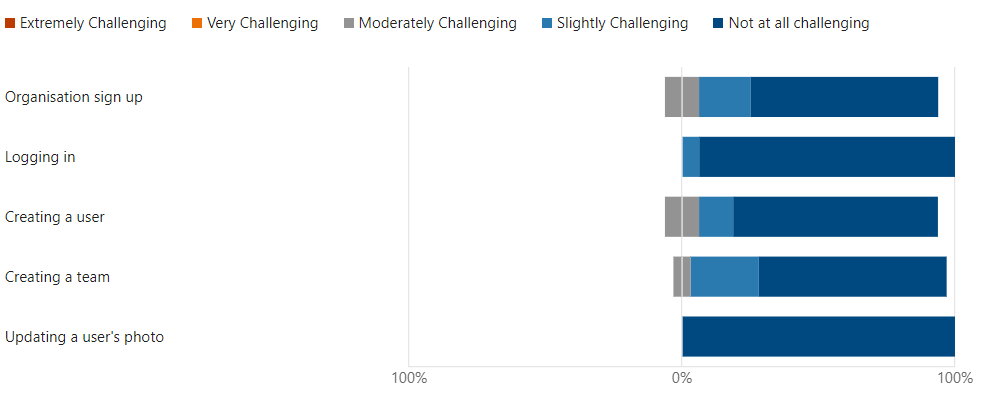
\includegraphics[scale=0.5]{dissertation/images/EvaluationAdminChallengingGraph.png}
\caption{Graph showing how challenging the participants found each task in the admin section}
\label{fig:admin task graph} 
\end{center}
\end{figure}

The additional feedback on the admin section also highlighted further themes to explore in future work. The participants appeared divided between liking and disliking the automated form feedback seen in \textbf{Fig. \ref{fig:admin form feedback}}, with one participant stating \textit{"Not a fan of the red outline and error messages under input elements immediately after going onto page. Would prefer if that happened upon a submission attemp[t] that fails validation"}. This feedback was initially designed to help the application conform to the visibility of system status and error prevention heuristics detailed in Jakob Nielsen's usability heuristics for user interface design (\cite{NeilsenHeuristics}), as messages inform users of optional and required fields as well as certain specifications that fields must meet. These feedback messages are updated on type, so will disappear once requirements are met. However, based on this feedback from the user evaluation, this feedback may conflict with the heuristic for aesthetic and minimalist design. User's opinions on this feature should be explored further in future evaluations as the current feedback is mixed.


\begin{figure}[h!]
\begin{center}
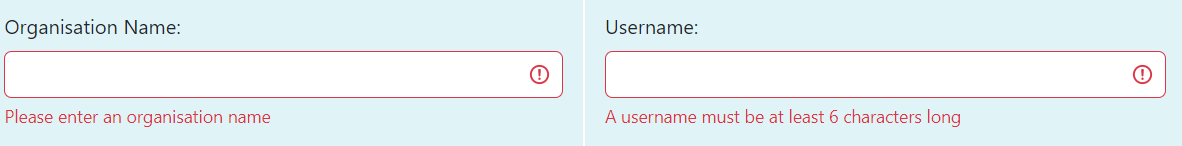
\includegraphics[scale=0.57]{dissertation/images/EvaluationExampleOfFormFeedback.png}
\caption{Example of the form feedback that divided user opinions}
\label{fig:admin form feedback} 
\end{center}
\end{figure}

Some workflow issues were also highlighted in the additional feedback section, with one user who had attempted to use the application before completing the survey. reporting being confused by the workflow. They had created an admin user and a team, and were confused as to why they kept getting 'unauthorised' errors when attempting to access the team's dashboards. Clearer unauthorised messages, mentioning the authorised user types, may have helped to resolve this misunderstanding, especially as a separate participant ran into a similar problem in the next section of tasks. This participant also mentioned that they would have expected read-only access to the team dashboards, which was overlooked when creating user permissions, but should certainly be included in future work. They also mentioned that earlier user acceptance testing would typically catch workflow issues like this. Unfortunately, due to project time constraints, this could not be completed in the current project timescale, but should be implemented in future development.

User interface feedback was also provided, with participants highlighting some scaling issues and suggesting alternatives to the window alerts currently in use. A large amount of positive feedback was also gathered here, with nine of the participants reporting that the admin side of the application was intuitive or easy to use, with one participant stating \textit{"The interface is overall very tidy and intuitive, but I particularly appreciated the design of the team member and team leader lists in the team overview, this made it very easy to see the participants and update them at a glance."} \\
\\
\textbf{Tags and Epics Dashboard Section}\\
From analysing \textbf{Fig \ref{fig:epic and tag form feedback}}, it can be seen that the majority of users found the 'adding a tag and value', 'creating an epic' and 'updating an epic/story' tasks to be not at all challenging. However, five of the sixteen participants found the 'creating a user story' task to be very or moderately challenging. To understand the reasoning behind this, the additional feedback responses were analysed. From here, it was discovered that seven of the participants struggled to find the button to add a story. The labelling of the button was deemed to be at fault. As can be seen in \textbf{Fig. \ref{fig:original vs new add story design}}, the original button does not specify it's purpose, an oversight in the design process, whereas the proposed new button style includes a label which will hopefully make its purpose clear to users. 

\begin{figure}[h!]
\begin{center}
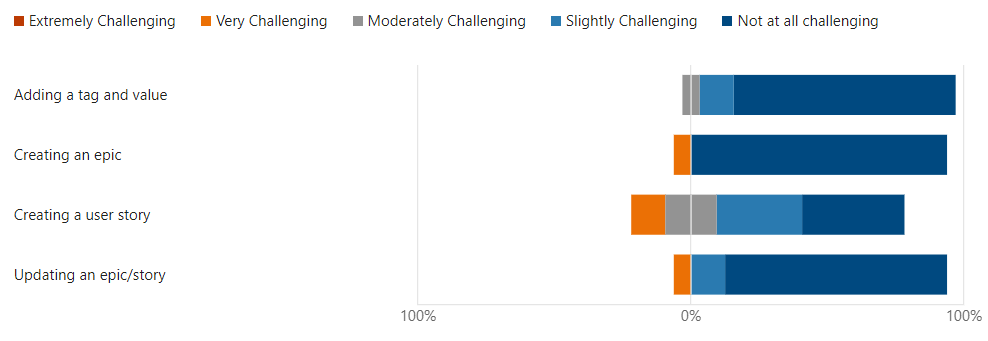
\includegraphics[scale=0.5]{dissertation/images/EvaluationEpicsAndTagsChallengingGraph.png}
\caption{Graph showing how challenging the participants found each task in the Epics and Tag Dashboard section}
\label{fig:epic and tag form feedback} 
\end{center}
\end{figure}

\begin{figure}[ht]
    \centering
    \subcaptionbox*{Original design}[.2\linewidth]{%
        \centering
        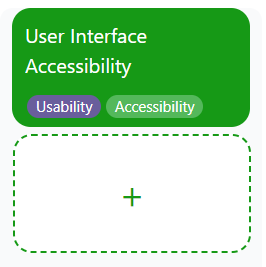
\includegraphics[width=\linewidth]{dissertation/images/EvaluationOriginalAddStoryButton.png}%
    }%
    \hspace{1em}
    \centering
    \subcaptionbox*{Proposed new design}[.2\linewidth]{%
        \centering
        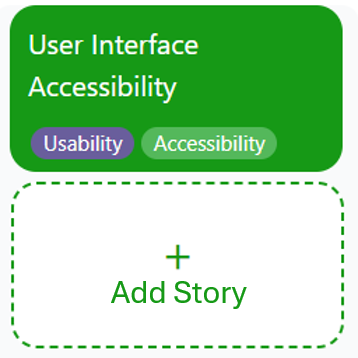
\includegraphics[width=\linewidth]{dissertation/images/EvaluationNewAddStoryButton.png}%
    }
    \caption{Original add story button design vs the proposed design change}
    \label{fig:original vs new add story design} 
\end{figure}


In \textbf{Fig. \ref{fig:epic and tag statement feedback}}, the participants were asked how much they agreed or disagreed with a set of statements surrounding the Epics and Tags Dashboard. The majority of these statements were mostly agreed or strongly agreed with by the participants. However, the statement 'the difference between tags and values is clear' was disagreed or strongly disagreed with by five participants. To understand why this was the case, the additional feedback examined. Here, three participants highlighted that example tags and values would be useful in order to further understand the different use cases of each element. Another user liked the descriptions on the Tag Dashboard before tags and values were added and suggested that they persisted even after actual elements were added. It was noticed throughout the survey responses that some of the participants were unlikely to have read the help documentation based on their responses to the survey questions. Due to the prevalence of this issue in the small-scale survey carried out, it is likely that this behaviour would also occur in real world use of the application. This poses a particular problem when creating more novel features, such as the introduction of business values, as the naive assumption was made that the developers would read the help documentation if they were confused on the differences between the tags and values. As this is unlikely to be typical user behaviour, the differences between these components needs to be more clearly highlighted in the Tag Dashboard itself, perhaps through the suggested addition of default tags and values, or a help tool tip which clearly describes the differences between the two functionalities. 

\begin{figure}[h!]
\begin{center}
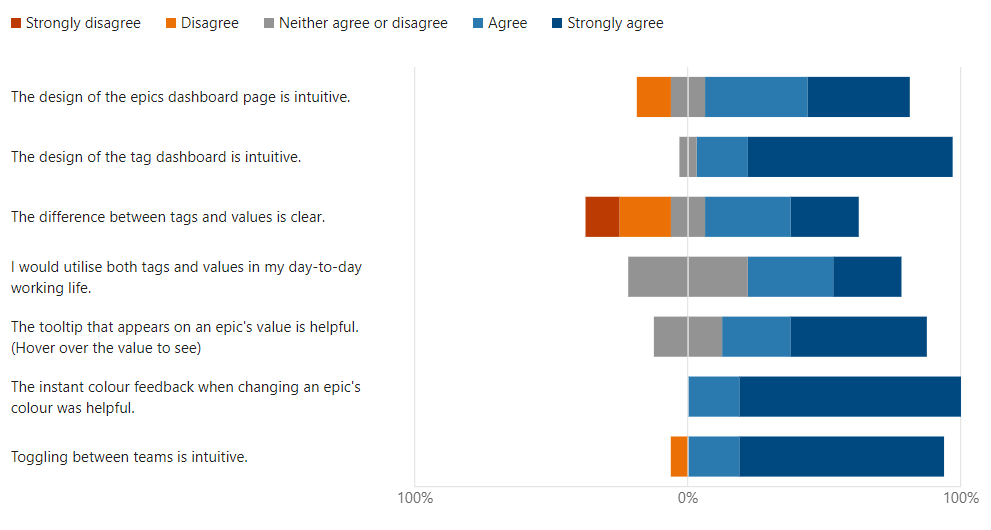
\includegraphics[scale=0.5]{dissertation/images/EvaluationEpicsAndTagsStatementGraph.png}
\caption{Graph showing how much a participant agreed or disagreed with the list of specified statements}
\label{fig:epic and tag statement feedback} 
\end{center}
\end{figure}

As seen in \textbf{Fig. \ref{fig:epic and tag statement feedback}}, seven participants neither agreed or disagreed with the statement 'I would utilise both tags and values in my day-to-day working life'. None of the additional feedback given expressly linked back to this statement. However, it is assumed that some of this reluctance comes from the ambiguous differentiation of the roles of tags and values. The importance of visible business value may also have been overlooked by developers, as this feature is not typically found in similar agile project management tooling. Part of the reason the value feature was added was also to help project stakeholders identify business values at a glance, without having to read full user stories. As no stakeholders were part of the evaluation process due to this functionality being a would have requirement, it was impossible to determine how useful this functionality would be deemed. As suggested future development includes creating this stakeholder view, further evaluation of the usefulness of the values functionality could be carried out after this has been implemented.

A large number of the participants gave extremely positive comments on the colour customisable components of the application. One participant stated \textit{"The option to freely colour-code is enormously helpful for me, especially with the instant updates in the interfaces. Not being confined to certain pre-set colours allows me to coordinate my records in RViT with external notes and colour schemes and is something I would utilise heavily in my day-to-day work"}. Another participant said \textit{"Moving the stories and epics is a great user experience. It works really well and the styling of it all including the columns slightly changing colour [on drag and drop] etc. is all fantastic."}. This feedback was extremely helpful as part of the reason for implementing this feature set was to compete with the less visually pleasing market-leading tools.

As with the previous task section, multiple user interface improvements were suggested. The most common suggestions involved repositioning buttons and added close buttons to the epic and story detail modals. \\
\\
\textbf{Tracking Dashboard Section}\\
As observed in \textbf{Fig. \ref{fig:tracking form feedback}}, the majority of participants found all four tasks in this section not at all challenging. However, four participants mentioned in the additional feedback section that the current method of editing a column's information, by clicking the title, did not seem very intuitive. This issue had also arisen in the pilot study where mouse-hover feedback was added in an attempt to make this functionality more apparent. Further improvements suggested in the feedback were to make the form appear when clicking anywhere on the column, or by introducing a new 'add stories' button or icon. Future work should include re-designing this form set up to be more intuitive to the user.

\begin{figure}[h!]
\begin{center}
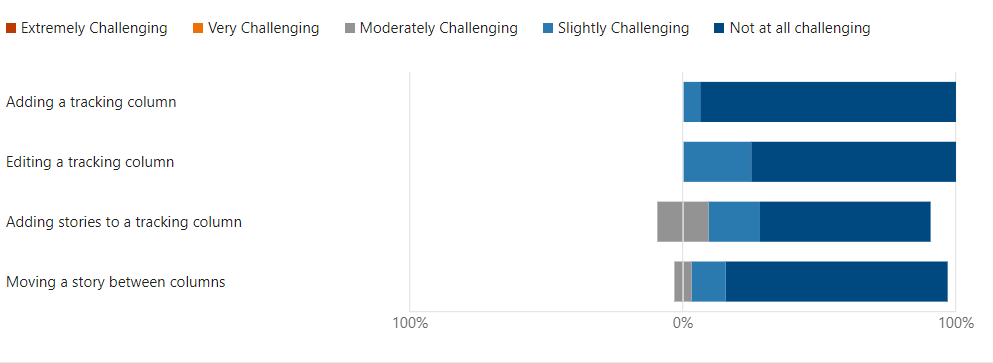
\includegraphics[scale=0.5]{dissertation/images/EvaluationTrackingChallengingGraph.png}
\caption{Graph showing how challenging the participants found each task in the Tracking Dashboard section}
\label{fig:tracking form feedback} 
\end{center}
\end{figure}

Valuable feedback was also given on the overall workflow of the Tracking dashboard. One participant suggested that a default flow should be created for newly defined teams. Two participants also suggested a more streamlined approach to adding stories to a column that had not previously been considered. They suggested that by adding a feature similar to the 'mark stories as complete' column option, users could choose to add all undefined user stories to a specified column. It was noted during development that the current manual adding of stories is not optimal, but this feature suggestion would automate this process.

As can be seen in \textbf{Fig. \ref{fig:tracking statement feedback}} the majority of participants either agreed or strongly agreed with all four statements specified. However, two participants disagreed that the time-based filters found on the Tracking Dashboard were intuitive. Only one participant mentioned this in their user feedback, stating that they were confused by the initial use of the filters, so had to read the help documentation to understand their purpose. While this demonstrates the helpfulness of the documentation provided, an on-page help feature, such as an on-hover tool tip could be implemented to explain the purpose of the filters. This would likely be helpful to new users, unfamiliar with similar tooling, as they could be overwhelmed by reading the full help documentation.

\begin{figure}[h!]
\begin{center}
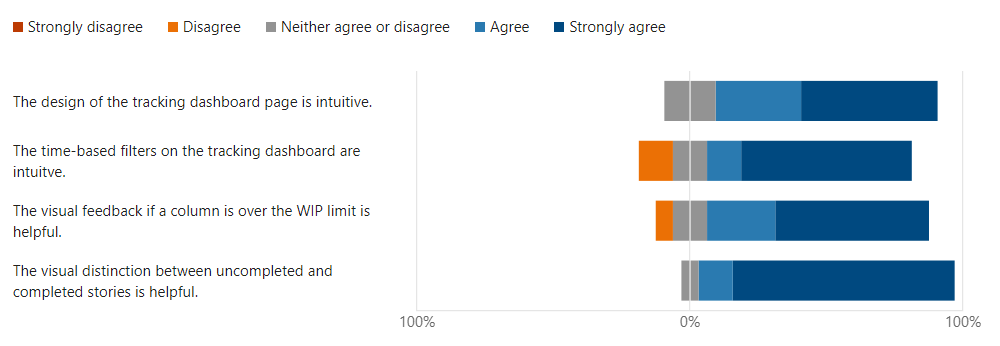
\includegraphics[scale=0.5]{dissertation/images/EvaluationTrackingStatementsGraph.png}
\caption{Graph showing how much a participant agreed or disagreed with the list of specified statements}
\label{fig:tracking statement feedback} 
\end{center}
\end{figure}

While the majority of users agreed or strongly agreed that the visual feedback displayed if a column is over the WIP limit is helpful, some of the participants did not feel that the change was bold enough. Some participants had also expected not to be allowed to move stories into a column if it was over the specified WIP limit. However, to maximise the flexibility of the application it was decided only to provide the visual feedback. One bug was also found in this section that had been missed during the testing phase. A user could not add a WIP limit of over 9 to a tracking column or an error message would pop up when the user tried to submit the form. This was unexpected behaviour, so the corresponding code was checked, and it was identified that the regex pattern specified on the input would only be valid for single digit. More thorough testing with special attention paid to edge cases could have caught this issue before the user evaluation was carried out.\\
\\
\textbf{Final Thoughts Section}\\
In this section a wide range of open-ended text responses were gathered. First the users were asked to compare RViT to other project management tools they had used in the past. The feedback here was very positive with half of the participants reporting that they found RViT easier to use or more intuitive than the industry-leading tool Jira, with one participant stating \textit{"RViT proved to be far simpler and more user-friendly compared to other tools I've used in the past, such as Jira. Although Jira offers numerous advantageous features and customisation possibilities, they can sometimes be overwhelming and require a significant amount of time to fully understand. On the other hand, with RViT, I was able to complete tasks swiftly and effectively, as its intuitive design made everything straightforward"}. Comparisons to Trello, another industry-leading tool, were made, with two of the participants stating that in its current form, RViT remains harder to use than Trello. It was highlighted by one of these participants that \textit{"A little more work on the whole end-to-end flow for a user would greatly enhance the experience"}. The inclusion of agile methodology and terminologies was also appreciated by the survey participants, with one stating \textit{"RViT was very intuitive, and I appreciated that it aligned with the terminology and categories of work items used in a software engineering context, a feature that many other tracking tools lack for me."}. Overall the feedback from this question was extremely helpful at identifying the strengths and weaknesses of RViT when compared to the industry standard tooling.

Many suggestions were made for possible future work, from proposed workflow improvements, such as thinking about how users could change roles during their time at an organisation, to future user interface work such as added dark mode functionality to the application. Further feature sets were also suggested, for example integrating RViT with other popular project management tooling such as GitHub, or adding collaboration features such as comments to the epics and user stories. It was also suggested to support other popular agile methodologies such as scrum as well as implementing calendar and scheduling components. Two participants also suggested creating an optional tutorial for new users to get them used to the application without having to read through the help documentation. Finally, one of the participants also suggested some small improvements to the in-app documentation to clearly define the roles of tags and values.

A wide variety of responses were collected in the final additional feedback question. Two participants mentioned that they liked the help documentation available on the application, with one saying \textit{"The documentation on the help page was excellent: Clearly structured, concise, and effective in explaining the system and its functionalities. Having it linked in the navigation made it easy to refer back to and enhanced the user experience."} while the other participant stated \textit{"The Help is pitched at the right level, allowing the user to quickly pick up what they need to know."}. Six of the twelve participants that responded to this question also highlighted that they liked the user interface design or experience with one participant stating \textit{"I really liked the application. I think it has a definite spot in the marketplace. It has a consistent design metaphor, it is easy and simple to use - this is its strength and the other available tools weakness"}. 


In total six distinct and replicable bugs were found in the user evaluation as detailed below:
\begin{itemize}
    \item Users were able to be registered with invalid email addresses.
    \item When adding or editing a user or team, it is possible to upload a text file in the photo section. It will tell you that file upload is successful, but the team/user will fail to be added/updated.
    \item An admin user is able to delete their account that is currently logged in and continue to have the ability to add to and edit the organisation's information.
    \item When setting an initial password for new users, this is displayed in plain text which is insecure.
    \item On the Tracking Dashboard users cannot add a WIP limit higher than 9 to a column.
    \item Some user interface scaling issues were noticed on smaller screens.
\end{itemize}
Asides from the user interface scaling issues, the majority of these bugs were oversights, and will easily be resolved through updating form validations. 


\subsection{Study Limitations}
While the user evaluation study highlighted key areas of RViT's success as an application as well as some of its weaknesses, it was fairly limited in scope. As previously mentioned, due to the reasonable time constraints set, the full functionality of the application could not be explored. The style of the evaluation also meant that participants were not able to experience using RViT in their day-to-day workflows but rather in the structured and tested workflow detailed in the survey. Future evaluations should endeavour to incorporate more flexibility of the use of RViT, perhaps with end goals established rather than a set task list.

There were also limitations in the diversity of the participants gathered. As mentioned in \textbf{Section 6.3.2}, all of the participants were experienced agile developers, with the majority having used similar tooling. Future evaluations looking at different user types would allow a nuanced look into how RViT handles users of different experience levels and highlight any improvements that could be made.

Another limitation was noticed when coding the qualitative responses. Many of the study participants did not fully explain the reasoning behind their responses, often only specifying that they did not like how a feature was currently implemented. This limited the amount of insight that was able to be gained from these responses. Future work could also incorporate semi-structured interviews or focus groups so that common issues could be further explored, and their root cause and solutions determined. 

\end{document}